% !TEX TS-program = pdflatex
% !TEX encoding = UTF-8 Unicode

% This is a simple template for a LaTeX document using the "article" class.
% See "book", "report", "letter" for other types of document.

\documentclass[11pt]{scrartcl} % use larger type; default would be 10pt

\usepackage[utf8]{inputenc} % set input encoding (not needed with XeLaTeX)

%%% Examples of Article customizations
% These packages are optional, depending whether you want the features they provide.
% See the LaTeX Companion or other references for full information.

%%% PAGE DIMENSIONS
\usepackage{geometry} % to change the page dimensions
\geometry{a4paper} % or letterpaper (US) or a5paper or....
\geometry{margin=1in} % for example, change the margins to 2 inches all round
% \geometry{landscape} % set up the page for landscape
%   read geometry.pdf for detailed page layout information

\usepackage{graphicx} % support the \includegraphics command and options

% \usepackage[parfill]{parskip} % Activate to begin paragraphs with an empty line rather than an indent

%%% PACKAGES
\usepackage{booktabs} % for much better looking tables
\usepackage{array} % for better arrays (eg matrices) in maths
\usepackage{paralist} % very flexible & customisable lists (eg. enumerate/itemize, etc.)
\usepackage{verbatim} % adds environment for commenting out blocks of text & for better verbatim
\usepackage{subfig} % make it possible to include more than one captioned figure/table in a single float
% These packages are all incorporated in the memoir class to one degree or another...

%%% HEADERS & FOOTERS
\usepackage{fancyhdr} % This should be set AFTER setting up the page geometry
\pagestyle{fancy} % options: empty , plain , fancy
\renewcommand{\headrulewidth}{0pt} % customise the layout...
\lhead{}\chead{}\rhead{}
\lfoot{}\cfoot{\thepage}\rfoot{}

%%% SECTION TITLE APPEARANCE
\usepackage{sectsty}
\allsectionsfont{\sffamily\mdseries\upshape} % (See the fntguide.pdf for font help)
% (This matches ConTeXt defaults)

%%% ToC (table of contents) APPEARANCE
\usepackage[nottoc,notlof,notlot]{tocbibind} % Put the bibliography in the ToC
\usepackage[titles,subfigure]{tocloft} % Alter the style of the Table of Contents
\renewcommand{\cftsecfont}{\rmfamily\mdseries\upshape}
\renewcommand{\cftsecpagefont}{\rmfamily\mdseries\upshape} % No bold!

%%% END Article customizations

%%% The "real" document content comes below...

\title{AC290 EXTREME COMPUTING: REPORT 1}
\subtitle{Bleeding Edge}
\author{Gioia Dominedo, Christian Junge, Abhishek Malali and Isadora Nun}
%\date{} % Activate to display a given date or no date (if empty),
         % otherwise the current date is printed 

\begin{document}
\maketitle

\section{What is the problem?}

The Influence Maximization Problem examines the behavior of nodes of a graph influencing one another.  For this assignment, we are looking at a graph of 240 nodes (representing individual Yelp reviewers) and the connections (edges) between them, and examining how the nodes within this graph activate one another.  The goal is to find the optimal set of starting nodes, that is, the set with the highest average number of nodes activated when the simulation is run repeatedly.  

\section{What is independent cascading?}

In the independent cascading approach, one or several nodes begin the simulation as activated.  In each iteration of the algorithm, each activated node has one chance to activate the nodes that are adjacent to it.  The probability that an activated node ($v$) will activate a node adjacent to it ($w$) is given by the Beta function with the parameters $\alpha$ and $\beta$, where $\alpha$ is the number of reviews that reviewer $w$ has written after reviewer $v$ (within a time frame given by $\tau$), and $\beta$ is the total number of reviews that reviewer $w$ has written.  Within the algorithm, this is implemented by selecting a random number from the Beta distribution and a random number from the Uniform distribution, and if the number from the Uniform distribution is less than the number from the Beta distribution, the node is activated.  Each node gets only one chance to activate its non-activated neighbors, and the independent cascade algorithm terminates when there are no more possibilities to activate further nodes.  The algorithm returns the total number of nodes that have been activated in the simulation.  

\section{What is the Influence function?}

The influence function is represented as follows:
\begin{equation}
f(S) = \frac{1}{N} \sum I(S)
\end{equation}

Where $N$ is the number of simulations, $f$ is the Influence function, $I$ is the independent cascade function, and $S$ is a given set of starting nodes.  The influence function tells the average number of nodes activated by a given set of starting nodes when the simulation is run N times, in other words the expected value of the number of activated nodes.  In the Influence Maximization Problem, we would like to find the set S of starting nodes that yields the highest value of the Influence function.    


\section{What is Greedy algorithm?}

The greedy algorithm runs a given number ($N$) of simulations, given a number of starting nodes.  In its first iteration, it finds the single node that has the highest expected value of activated nodes when run over $N$ simulations.  In each subsequent iteration, it finds the next node which, when added to the starting set, returns the highest expected value of activated nodes when run over $N$ simulations.  In this way, additional starting nodes are incrementally added to the set which was previously determined to be the best set until the set contains the desired number of starting nodes.  
	
The danger in this approach is that a set of n starting nodes may be the best n-element sized set of starting nodes, but the best set of nodes that is created by adding one more element to size-n set may not be the best size(n+1) set possible.  

\begin{figure}[h!]
\centering
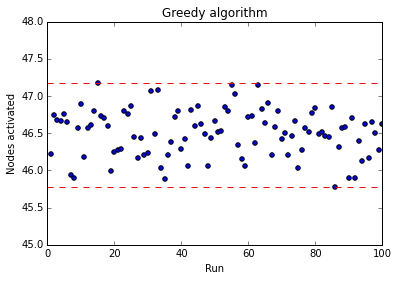
\includegraphics[width=10 cm]{Greedy}
%\label{fig_sim}
\caption{Greedy algorithm}
\label{fig:GA}
\end{figure}

As we can see in figure \ref{fig:GA}, the results for 100 runs of the greedy algorithm for the mini North Carolina graph ($N=1000$) are in a tight range between 45.77 and 47.17. We obtain a ratio $f_{min}/f_{max} = 0.97$. We believe that $N=1000$ is big enough to minimize the uncertainties on the results. 

\section{What is Simulated Annealing?}

Simulated Annealing is a process to stochastically find the optimal starting set of nodes.  This optimization process is used for discrete search spaces where an exhaustive search would take a prohibitively long time.  In the case of the Maximum Influence Problem, testing all possible combinations of nodes would take a very long time, so simulated annealing is a sensible approach.  For this problem, the goal is to find the set of starting nodes with the highest value of the influence function; in other words, the set of starting nodes with the highest expected number of activated nodes.  

The process works as follows: First, an initial set is selected and the expected value of activated nodes for a given number of simulations is calculated.  Then this starting set is perturbed (for example, by switching some of the starting nodes), and the expected value of this new set is calculated.  If this new set yields a higher expected value, then it is accepted, but if this new set yields a lower expected value, then it is accepted with a probability based on the temperature ($P(X=j)=\exp({\frac{-\Delta E}{T}})$).  This process runs over many iterations, yielding a set that returns the highest expected value of activated nodes.  

In the simulated annealing process as in the greedy algorithm, there remains the potential that the actual optimal solution is not found because the set is “stuck” with some nodes that yield good intermediate results when included in the set, but are not the best overall.  For this reason, the concept of “heat” is introduced into the annealing process.  This works as follows:  
If the new starting set returns an expected value that is much higher (“higher” is relative, and can be calibrated in the algorithm), then the number of starting nodes that are switched in subsequent runs of the influence function is kept the same (or potentially increased).  This is referred to as “heat”, and determines how drastic of a change is made to the considered set of starting nodes at each step in the simulated annealing process. In contrast, if the expected value is not much higher, the algorithm “cools”, and fewer nodes are switched.  Periodically, the algorithm is “heated up” to stimulate it to make more drastic changes to ensure that it is not stuck in a relative maximum that is lower than the absolute maximum.  

Over many iterations, the simulated annealing process should yield the set of points with the highest expected value of activated nodes. 

\begin{figure}[h!]
\centering
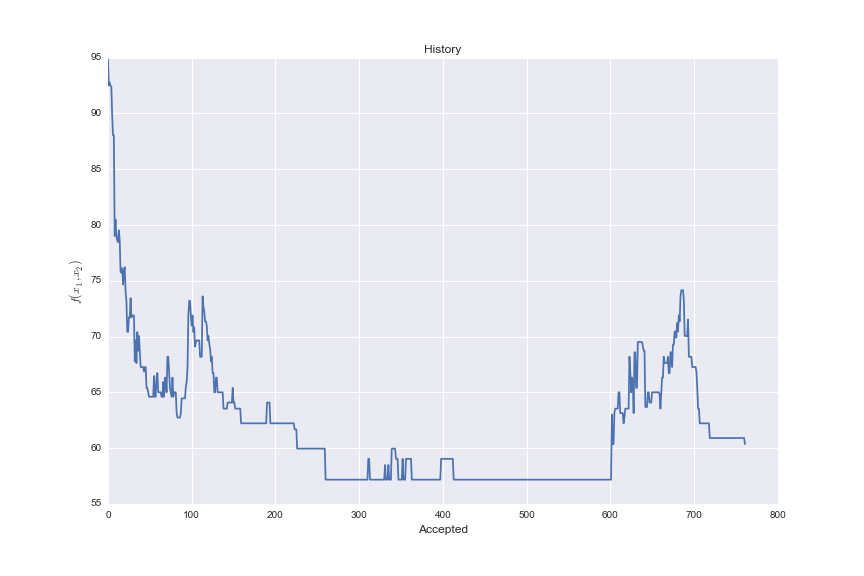
\includegraphics[width=10 cm]{SimAn}
%\label{fig_sim}
\caption{Simulated Annealing}
\label{fig:SA}
\end{figure}

\section{Uncertainties in the optimization}

Uncertainty in the optimization results from stochastic approaches, which yield estimates with an unknown amount of error rather than definite values.  In particular, the influence function returns an expected value that has a certain amount of uncertainty.  While the standard error of the independent cascade function is endemic to a given set of starting nodes, regardless of the number of simulations, the standard error of the Influence function shrinks as the number of independent cascade simulations ($N$) increases.  Therefore, a larger number of simulations will yield a more accurate estimate of the average influence for a given set.  We see that this tightening of the standard error is proportional to $\frac{\alpha}{N^{\lambda}}$. By fitting the data with a linear regression we obtain  $\frac{11.34}{N^{0.46}}$   So any optimization algorithm using the influence function will be impacted by its inherent uncertainty, which can only be reduced by increasing the number of simulations.  
	
\begin{figure}
\centering
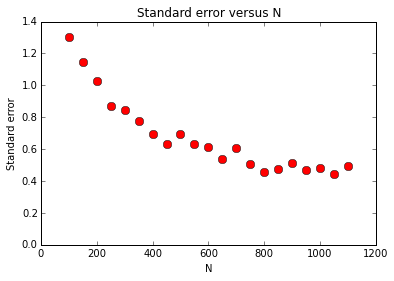
\includegraphics[width=10 cm]{StandardErrorVsN}
%\label{fig_sim}
\caption{Standard error versus N}
\label{fig:StandardError}
\end{figure}

\begin{figure}
\centering
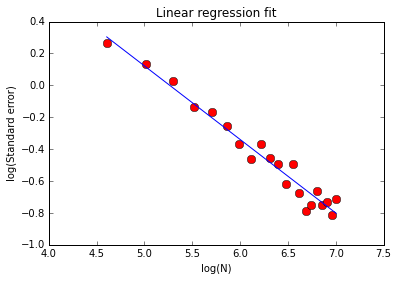
\includegraphics[width=10 cm]{LinearR}
%\label{fig_sim}
\caption{Standard error versus N}
\label{fig:LR}
\end{figure}
	 
\begin{figure}
\centering
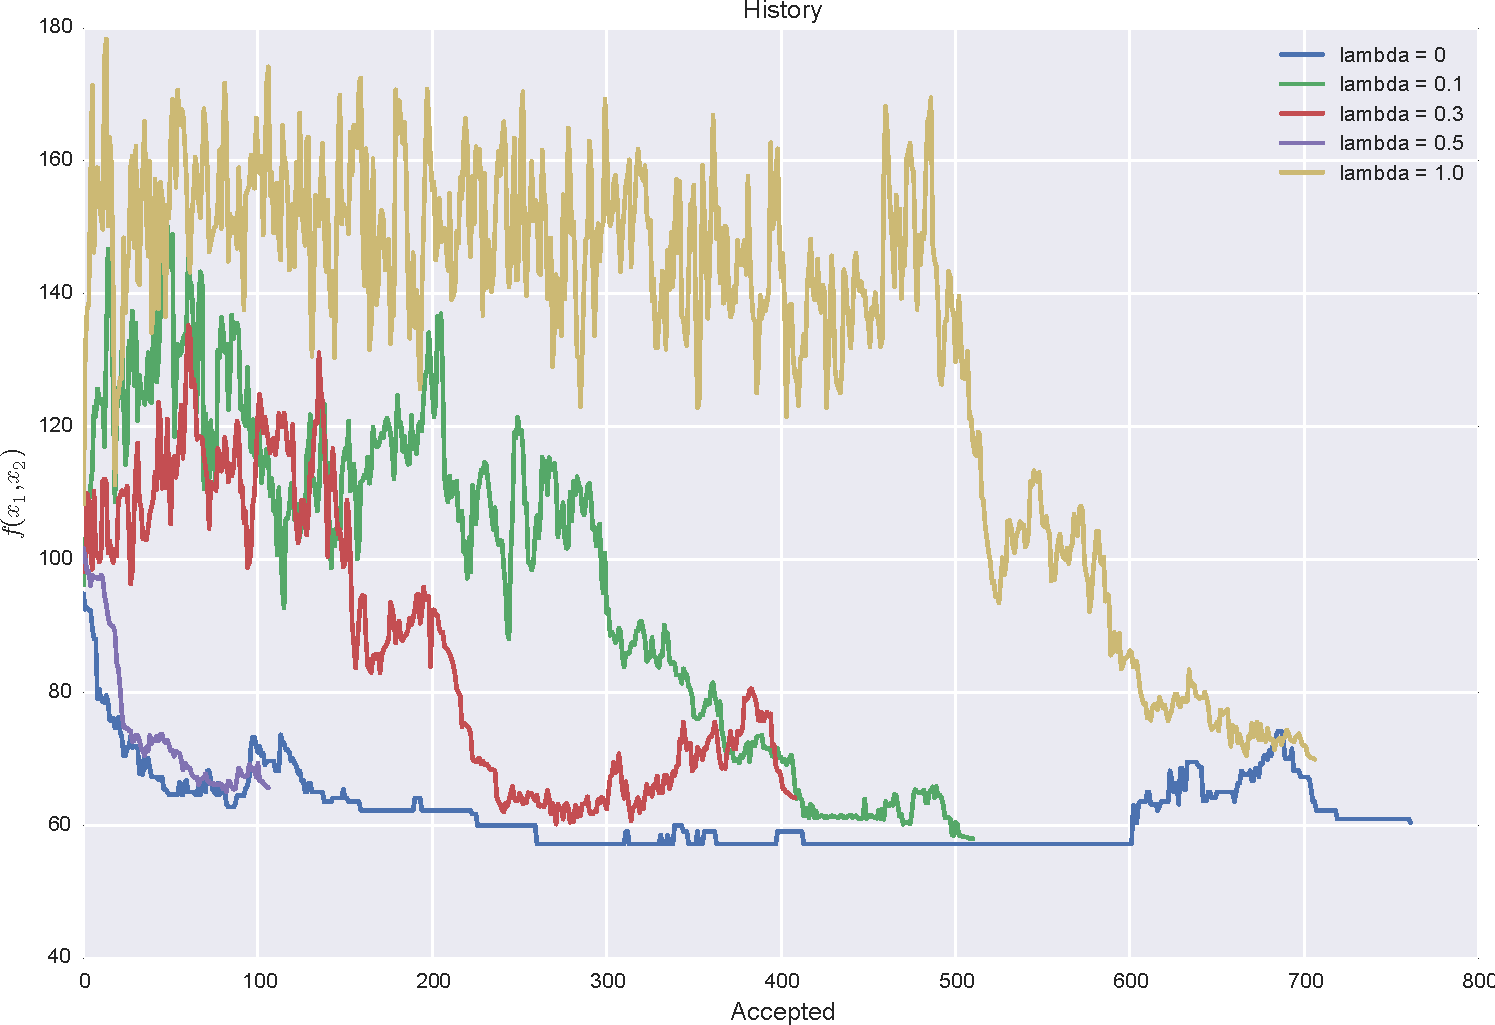
\includegraphics[width=10 cm]{lambda01}
%\label{fig_sim}
\caption{Simulated annealing with noise $= \lambda*random.uniform(0,1)$ for different values of $\lambda$}
\label{fig:SA}
\end{figure}
	 

\end{document}
